\documentclass[xcolor=dvipsnames]{beamer}
\usepackage[T1]{fontenc}
\usepackage[utf8]{inputenc}
\usepackage[english,slovak]{babel}

\usepackage{amsmath}
\usepackage{amsthm}
\usetheme{Pittsburgh}
\useoutertheme{shadow}

\usepackage{graphicx}
\usepackage{caption}
\usepackage{subcaption}

\usepackage[]{algorithm2e}
\usepackage{listings}
 \setbeamercovered{transparent}
 \usepackage{cuted}
\usepackage[export]{adjustbox}
\usepackage{mathtools}

\usepackage{lipsum}
\usepackage{verbatim}

\newcommand\Wider[2][3em]{%
\makebox[\linewidth][c]{%
  \begin{minipage}{\dimexpr\textwidth+#1\relax}
  \raggedright#2
  \end{minipage}%
  }%
}




\iftrue

\usetheme{Warsaw}

\setbeamercolor{normal text}{fg=white,bg=black!90}
\setbeamercolor{structure}{fg=white}

\setbeamercolor{alerted text}{fg=red!85!black}

\setbeamercolor{item projected}{use=item,fg=black,bg=item.fg!35}

\setbeamercolor*{palette primary}{use=structure,fg=structure.fg}
\setbeamercolor*{palette secondary}{use=structure,fg=structure.fg!95!black}
\setbeamercolor*{palette tertiary}{use=structure,fg=structure.fg!90!black}
\setbeamercolor*{palette quaternary}{use=structure,fg=structure.fg!95!black,bg=black!80}

\setbeamercolor*{framesubtitle}{fg=white}

\setbeamercolor*{block title}{parent=structure,bg=black!60}
\setbeamercolor*{block body}{fg=black,bg=black!10}
\setbeamercolor*{block title alerted}{parent=alerted text,bg=black!15}
\setbeamercolor*{block title example}{parent=example text,bg=black!15}

\fi



%-------------------------------------------------------------------------------------
\title{\bf Dense convolutional neural network in embedded systems}
\author{Michal CHOVANEC, PhD}


%\setbeamertemplate{footline}[frame number]{}
\setbeamertemplate{navigation symbols}{}


\date[EURP]{}
\begin{document}

\begin{frame}
\titlepage


\begin{columns}
\begin{column}{0.5\textwidth}

  \begin{figure}
    
\includegraphics[scale=0.15]{../../pictures/arm_cortex.jpg}
  \end{figure}

\end{column}
\begin{column}{0.5\textwidth}  %%<--- here

  \begin{figure}
  
\includegraphics[scale=0.1]{../../pictures/nvidia.png}
  \end{figure}

\end{column}
\end{columns}

\end{frame}


\begin{frame}{\bf Motivation}


\begin{columns}
\begin{column}{0.5\textwidth}

\begin{itemize}
  \item build smarter robots
  \item embedded particle filtering
  \item embedded localization
  \item embedded decision making
\end{itemize}

\end{column}
\begin{column}{0.5\textwidth}  %%<--- here

\begin{itemize}
  \color{red}
  \item only one MCU
  \item no C++ libs
  \item obsolete architectures
  \item float instead of int
\end{itemize}

\end{column}
\end{columns}


  \begin{figure}
    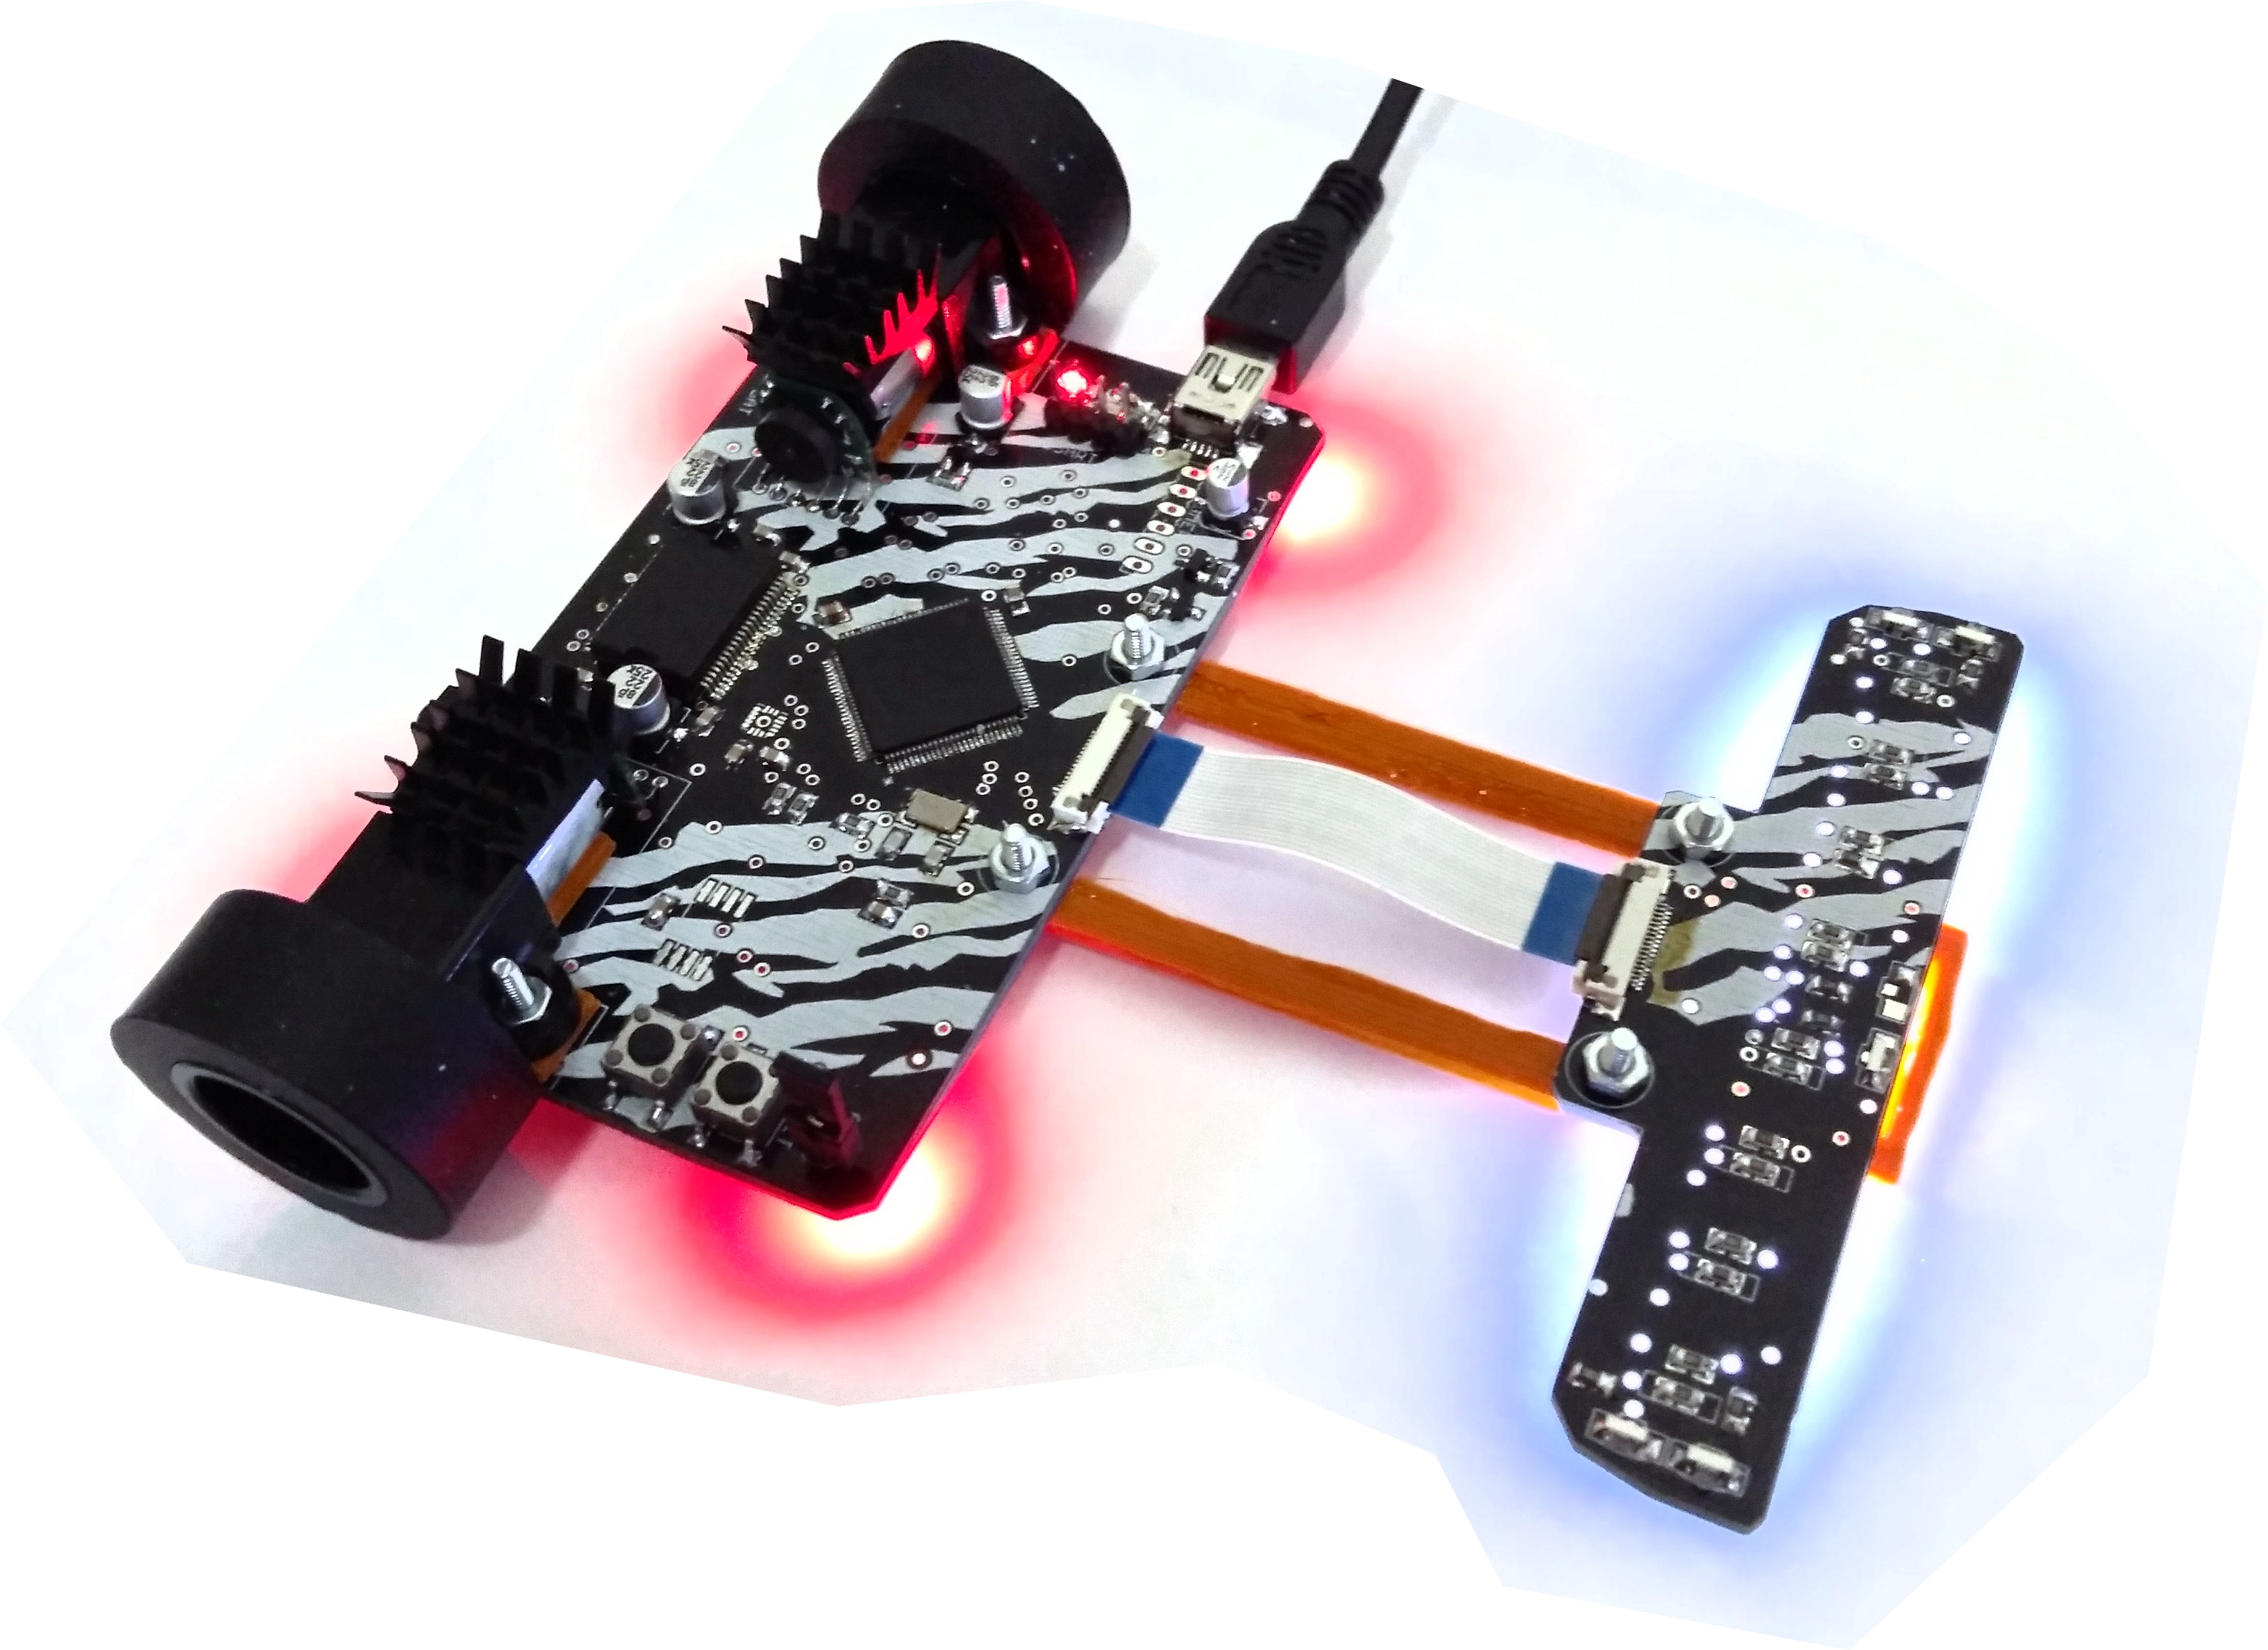
\includegraphics[scale=0.07]{../../pictures/robot_ascender.jpg}
  \end{figure}


\end{frame}



\begin{frame}{\bf Motivation}

\begin{itemize}
  \item line type classification
  \item prediction curve type
  \item predictive braking
  \item map creating
\end{itemize}

  \begin{figure}
    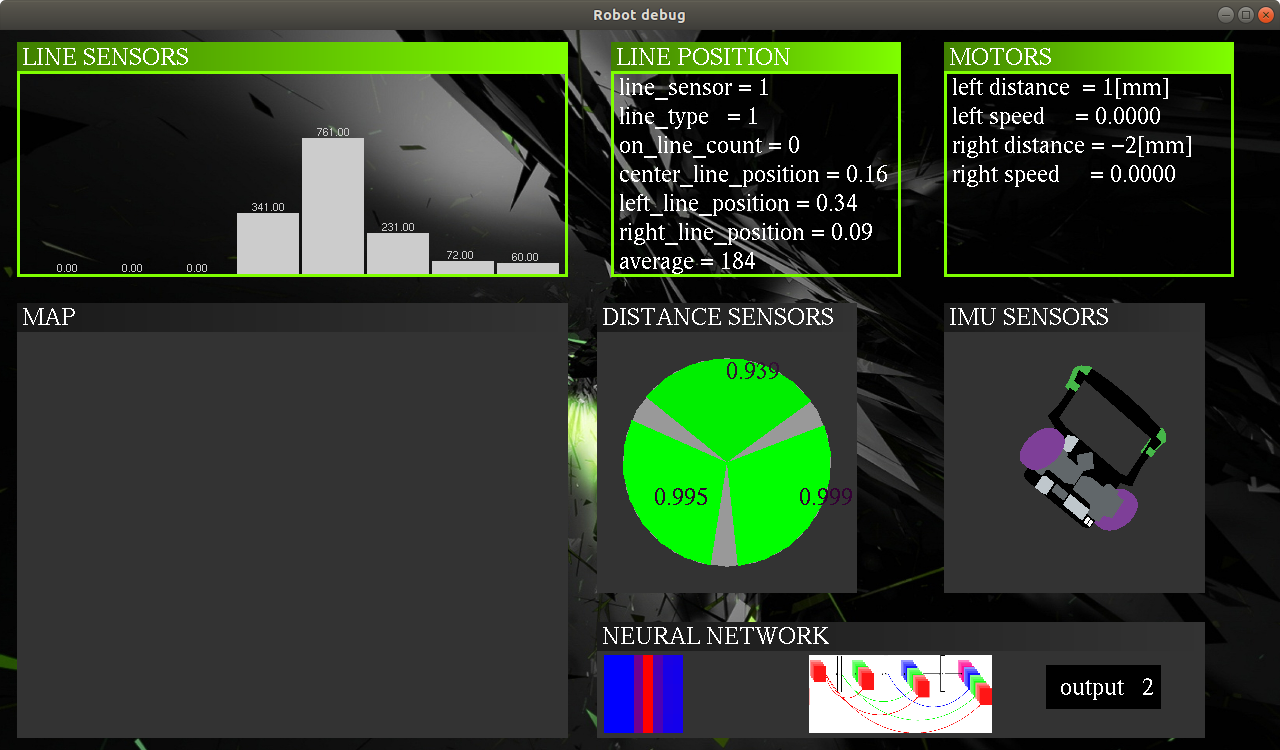
\includegraphics[scale=0.2]{../../pictures/robot_debug_app.png}
  \end{figure}


\end{frame}


\begin{frame}{\bf Target hardware}

\begin{table}[]
\begin{tabular}{|c|c|c|c|}
\hline
target                                                       & bits & features                                                                 & frequency                                              \\ \hline
\begin{tabular}[c]{@{}c@{}}AVR\\ Atmega 328\end{tabular}     & 8    & single cycle ADD, MUL                                                    & 20MHz                                                  \\ \hline
\begin{tabular}[c]{@{}c@{}}ARM \\ Cortex M0\end{tabular}     & 32   & single cycle ADD, MUL                                                    & 48MHz                                                  \\ \hline
\begin{tabular}[c]{@{}c@{}}ARM \\ Cortex M4, M7\end{tabular} & 32   & \begin{tabular}[c]{@{}c@{}}SIMD DUAL 16bit MAC \\ , FPU ...\end{tabular} & \begin{tabular}[c]{@{}c@{}}72MHz\\ 216MHz\end{tabular} \\ \hline
\end{tabular}
\end{table}


\end{frame}



\begin{frame}{\bf Convolutional neural network}


\begin{figure}
  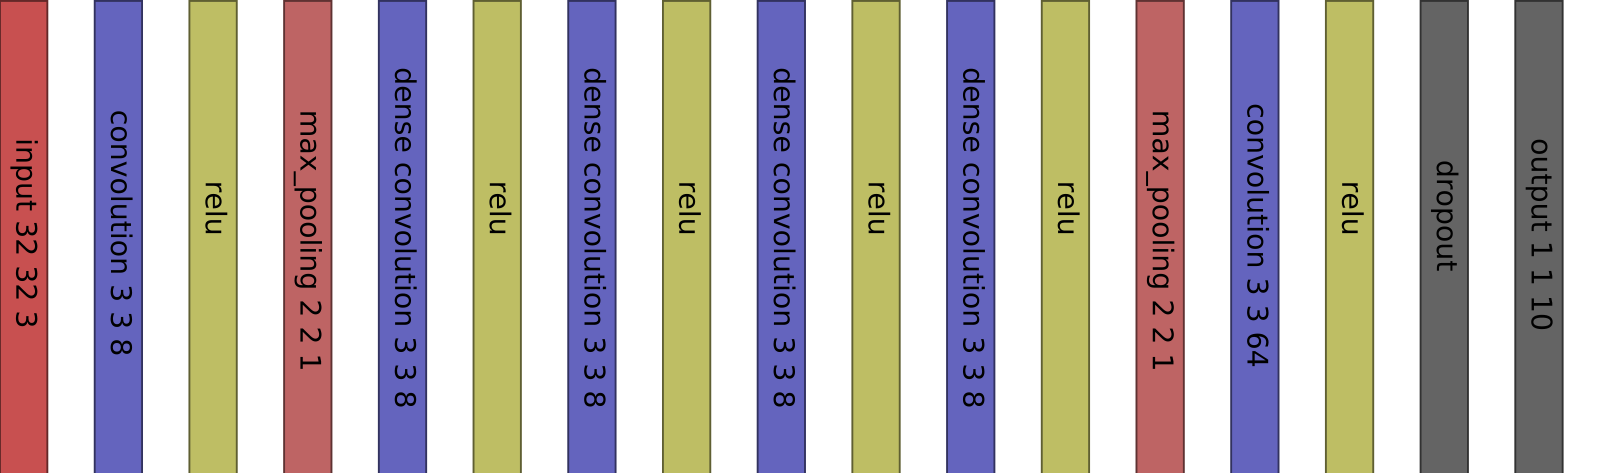
\includegraphics[scale=0.2]{../../diagrams/cnn_architecture_example.png}
\end{figure}


\begin{itemize}
  \item input tensor (image)
  \item convolutional layer
  \item dense convolutional layer
  \item relu layer (nonlinearity)
  \item pooling layer
  \item full connected layer
\end{itemize}


\end{frame}


\begin{frame}[fragile]
{\bf Discrete convolution}

\begin{figure}
  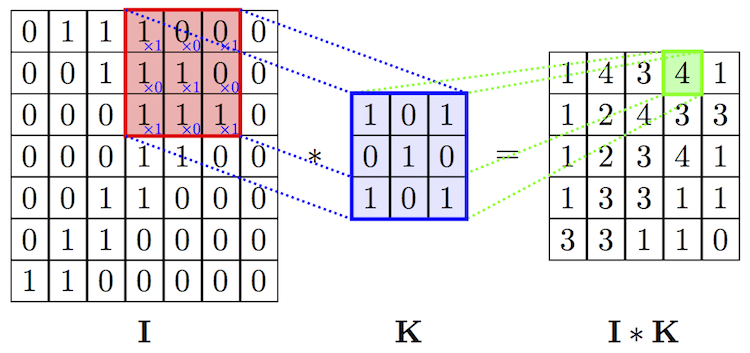
\includegraphics[scale=0.2]{../../diagrams/convolution_2d.png}
\end{figure}

\lstset{language=C++,
                basicstyle=\tiny,
                emph={int,char,double,float,unsigned},
                emphstyle={\color{blue}},
                numberstyle=\color{green}\tiny,
                keywordstyle=\color{red}\bf\ttfamily,
                stringstyle=\color{red}\ttfamily,
                commentstyle=\color{green}
}

\begin{lstlisting}

for (unsigned y = 0; y < input_height; y++)
for (unsigned x = 0; x < input_width; x++)
{
    float sum = 0.0;

    for (unsigned ky = 0; ky < kernel_height; ky++)
    for (unsigned kx = 0; kx < kernel_width; kx++)
    {
      sum+= kernel[ky][kx]*input[y + ky][x + kx];
    }

    output[y + kernel_height/2][x + kernel_width/2] = sum;
  }
}
\end{lstlisting}
\end{frame}




\begin{frame}[fragile]
{\bf Activation function}

tanh, sigmoid, gaussian, {\bf RELU}, leaky RELU ...
\begin{figure}
  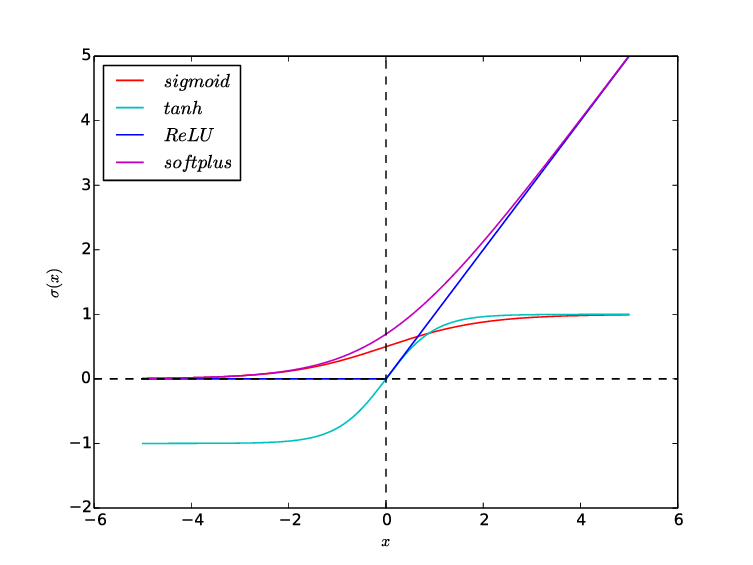
\includegraphics[scale=0.2]{../../pictures/activation.png}
\end{figure}

\begin{columns}
\begin{column}{0.5\textwidth}
\[ f(x) =
  \begin{cases}
    x       & \quad \text{if } x > 0\\
    0       & \quad \text{otherwise}
  \end{cases}
\]
\end{column}
\begin{column}{0.5\textwidth}  %%<--- here
\[ \frac{df(x)}{dx} =
  \begin{cases}
    1       & \quad \text{if } x > 0\\
    0       & \quad \text{otherwise}
  \end{cases}
\]
\end{column}
\end{columns}

\end{frame}


\begin{frame}{\bf Pooling}

\begin{figure}
  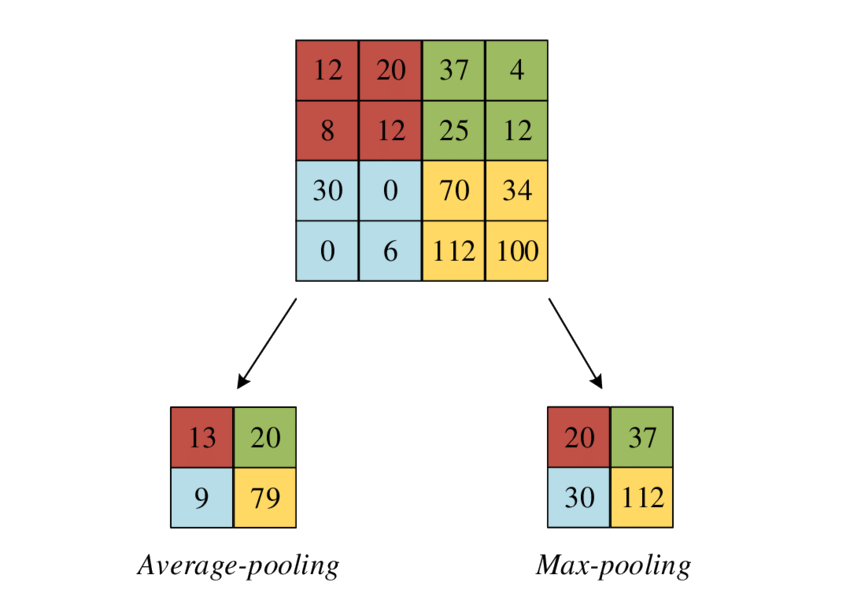
\includegraphics[scale=0.2]{../../diagrams/pooling.png}
\end{figure}

\end{frame}


\begin{frame}{\bf Convolutional neural network - CNN}

  \begin{figure}
    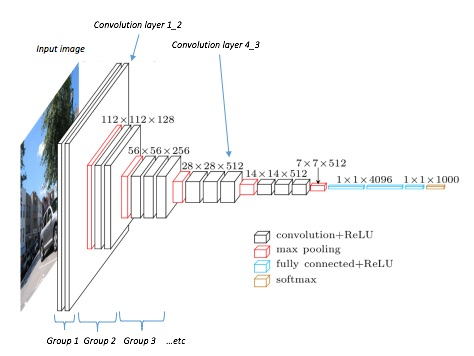
\includegraphics[scale=0.5]{../../diagrams/cnn.jpg}
  \end{figure}

\end{frame}


\begin{frame}{\bf Dense CNN}


State of the art in image recognition.


\begin{table}[]
\begin{tabular}{|l|l|l|l|l|}
\hline
\textbf{architecture}                                              & \textbf{depth} & \textbf{params} & \textbf{CIFAR 10} & \textbf{CIFAR 100} \\ \hline
ResNet                                                             & 110            & 1.7M            & 13.63\%           & 44.74\%            \\ \hline
\begin{tabular}[c]{@{}l@{}}ResNet \\ Stochastic Depth\end{tabular} & 110            & 1.7M            & 11.66\%           & 37.8\%             \\ \hline
DenseNet k = 12                                                    & 40             & 1.0M            & \textbf{7.0\%}    & \textbf{27.55\%}   \\ \hline
DenseNet k = 24                                                    & 100            & 27.2M           & \textbf{5.83\%}   & \textbf{23.42\%}   \\ \hline
\end{tabular}
\end{table}

  \begin{figure}
    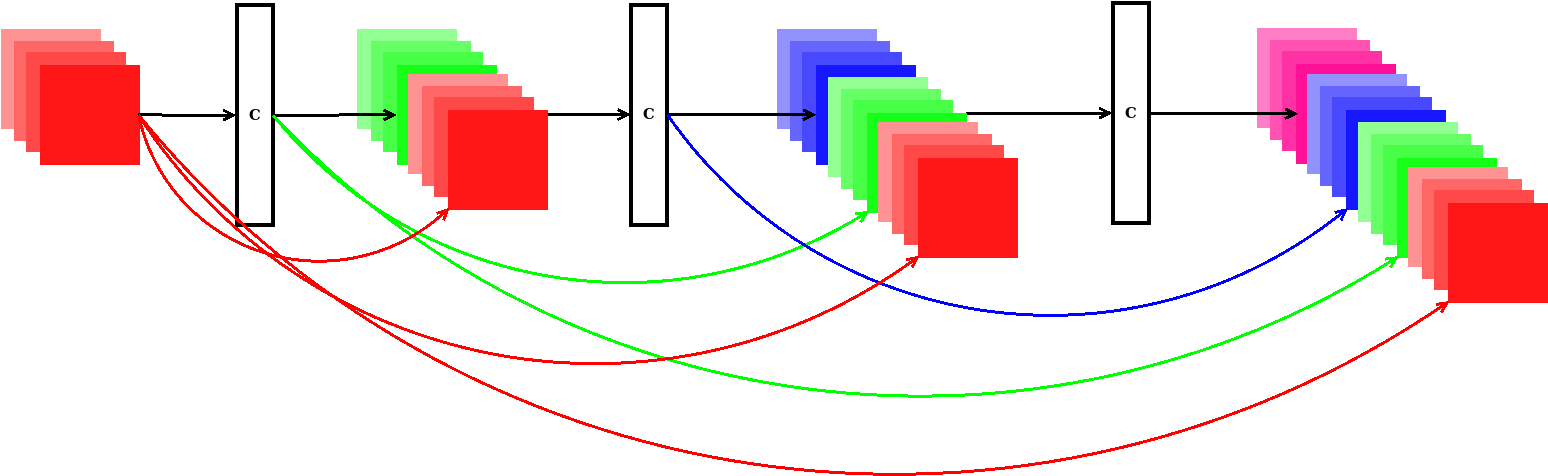
\includegraphics[scale=0.2]{../../diagrams/dense_net.png}
  \end{figure}


\end{frame}


\begin{frame}{\bf Network example - MNIST handwritten digits recognition}



\begin{columns}
\begin{column}{0.5\textwidth}

\begin{itemize}
  \item training count 50000
  \item testing count 10000
  \item input size 28x28x1 pixels
\end{itemize}

\end{column}
\begin{column}{0.5\textwidth}  %%<--- here

\begin{figure}
  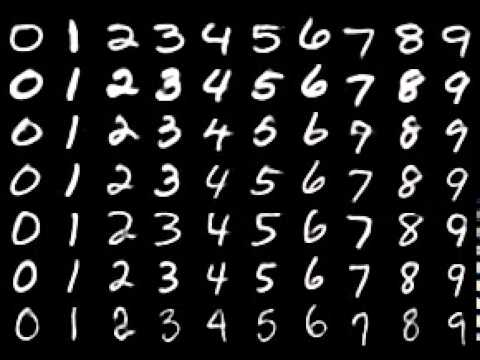
\includegraphics[scale=0.2]{../../pictures/mnist.jpg}
\end{figure}

\end{column}
\end{columns}

Tested architecture

C8 - P2 - D8 - D8 - P2 - D8 - D8 - D8 - D8 - FC

\begin{figure}
  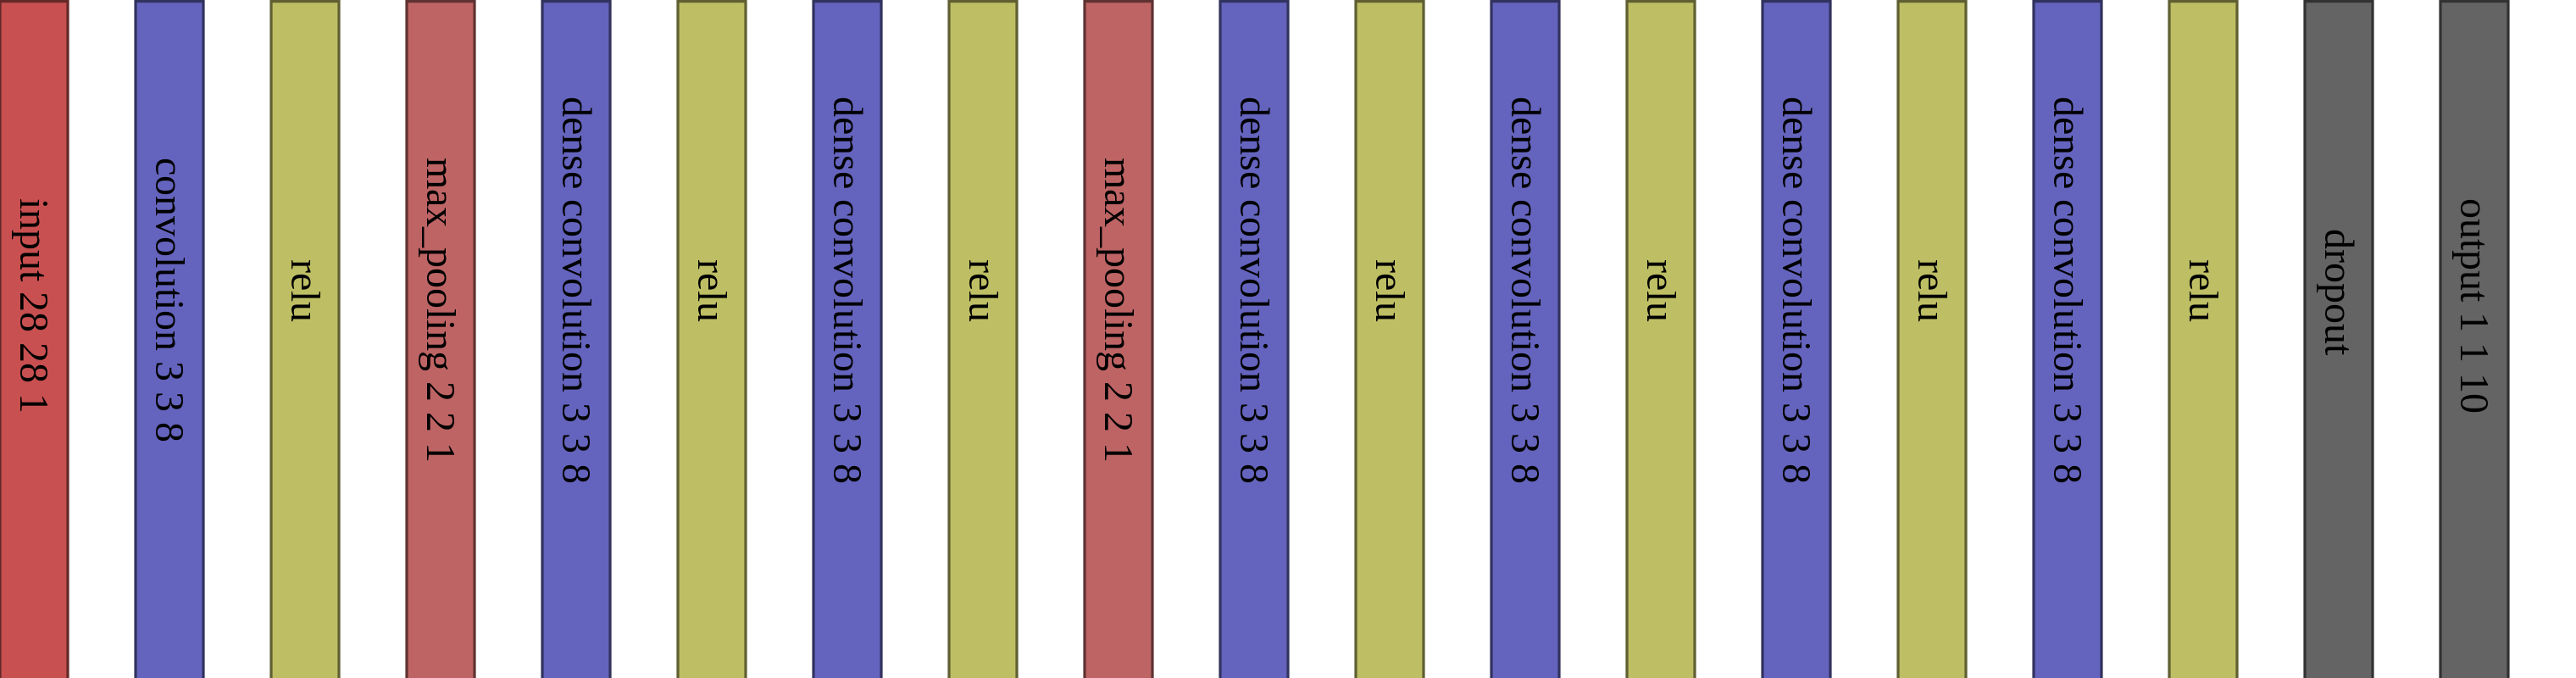
\includegraphics[scale=0.14]{../../diagrams/cnn_architecture.png}
\end{figure}

\end{frame}


\begin{frame}[fragile]
{\bf Training result}

Network success rate - confusion matrix

{\tiny
  \begin{verbatim}
  976        0        1        0        1        1        6        0        1        1
    1     1129        0        0        0        0        3        3        0        0
    1        3     1028        1        0        0        0        6        1        1
    0        0        0      995        0        4        0        0        0        1
    0        0        0        0      973        0        1        0        2        7
    0        1        0        4        0      885        2        0        1        5
    0        0        1        0        1        1      942        0        0        0
    1        1        1        6        1        1        0     1018        0        6
    1        1        1        3        0        0        4        1      967        1
    0        0        0        1        6        0        0        0        2      987

  99.592   99.471   99.612   98.515   99.084   99.215    98.33   99.027   99.281    97.82


  9900      100       99%
  \end{verbatim}
}

\end{frame}




\begin{frame}{\bf Embedded network implementation}

convert float weights to int8\_t
\begin{align*}
  scale &= max{(|\vec{w}|_1)} \\
  \vec{w}' &= \vec{w}\frac{127}{scale}
\end{align*}


use double buffer memory trick

\begin{itemize}
  \item unsigned buffer\_size = $\max_{i}$(layers[i].input\_size());
  \item buffer\_a = new int8\_t(buffer\_size);
  \item buffer\_b = new int8\_t(buffer\_size);
\end{itemize}

\begin{figure}
  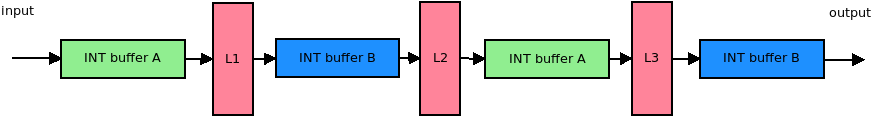
\includegraphics[scale=0.3]{../../diagrams/nn_memory.png}
\end{figure}

\end{frame}


\begin{frame}[fragile]
{\bf Optimize kernel - templates}

\lstset{language=C++,
                basicstyle=\tiny,
                emph={int,char,double,float,unsigned},
                emphstyle={\color{blue}},
                numberstyle=\color{green}\tiny,
                keywordstyle=\color{red}\bf\ttfamily,
                stringstyle=\color{red}\ttfamily,
                commentstyle=\color{green}
}

\begin{lstlisting}

templete<unsigned int kernel_size>
void convolution()
{
  for (unsigned y = 0; y < input_height; y++)
  for (unsigned x = 0; x < input_width; x++)
  {
      int sum = 0;

      for (unsigned ky = 0; ky < kernel_size; ky++)
      for (unsigned kx = 0; kx < kernel_size; kx++)
      {
        sum+= kernel[ky][kx]*input[y + ky][x + kx];
      }

      output[y + kernel_size/2][x + kernel_size/2] = (sum*scale)/127;
    }
  }
}
\end{lstlisting}
\end{frame}





\begin{frame}[fragile]
{\bf Optimize kernel - unrolling}

\lstset{language=C++,
                basicstyle=\tiny,
                emph={int,char,double,float,unsigned},
                emphstyle={\color{blue}},
                numberstyle=\color{green}\tiny,
                keywordstyle=\color{red}\bf\ttfamily,
                stringstyle=\color{red}\ttfamily,
                commentstyle=\color{green}
}

\begin{lstlisting}

templete<unsigned int kernel_size>
void convolution()
{
  for (unsigned y = 0; y < input_height; y++)
  for (unsigned x = 0; x < input_width; x++)
  {
      int sum = 0;

      if (kernel_size == 3)
      {
        sum+= kernel[0][0]*input[y + 0][x + 0];
        sum+= kernel[0][1]*input[y + 0][x + 1];
        sum+= kernel[0][2]*input[y + 0][x + 2];

        sum+= kernel[1][0]*input[y + 1][x + 0];
        sum+= kernel[1][1]*input[y + 1][x + 1];
        sum+= kernel[1][2]*input[y + 1][x + 2];

        sum+= kernel[2][0]*input[y + 2][x + 0];
        sum+= kernel[2][1]*input[y + 2][x + 1];
        sum+= kernel[2][2]*input[y + 2][x + 2];
      }

      output[y + kernel_size/2][x + kernel_size/2] = (sum*scale)/127;
    }
  }
}
\end{lstlisting}

{\bf 3.6x speed up}

\end{frame}


\begin{frame}[fragile]
{\bf Optimize kernel - SIMD}


\lstset{language=C++,
                basicstyle=\small,
                emph={int,char,double,float,unsigned},
                emphstyle={\color{blue}},
                numberstyle=\color{green}\tiny,
                keywordstyle=\color{red}\bf\ttfamily,
                stringstyle=\color{red}\ttfamily,
                commentstyle=\color{green}
}

\begin{lstlisting}

sum+= kernel[0][0]*input[y + 0][x + 0];
sum+= kernel[0][1]*input[y + 0][x + 1];
sum+= kernel[0][2]*input[y + 0][x + 2];


smlabb	r2, fp, sl, r2
ldrsb.w	sl, [r8, #1]
ldrsb.w	fp, [r0, #-24]

smlabb	r2, fp, sl, r2
ldrsb.w	sl, [r8, #2]
ldrsb.w	fp, [r0, #-23]

smlabb	r2, fp, sl, r2
ldrsb.w	sl, [r8, #3]
ldrsb.w	fp, [r0, #-22]

\end{lstlisting}


\end{frame}


\begin{frame}{\bf Results}

\begin{itemize}
\item float network accuracy 99\%
\item int8 network accuracy  98.97\%
\item runtime on 216MHz Cortex M7 18ms (72Mop/s)
\end{itemize}

\begin{figure}
  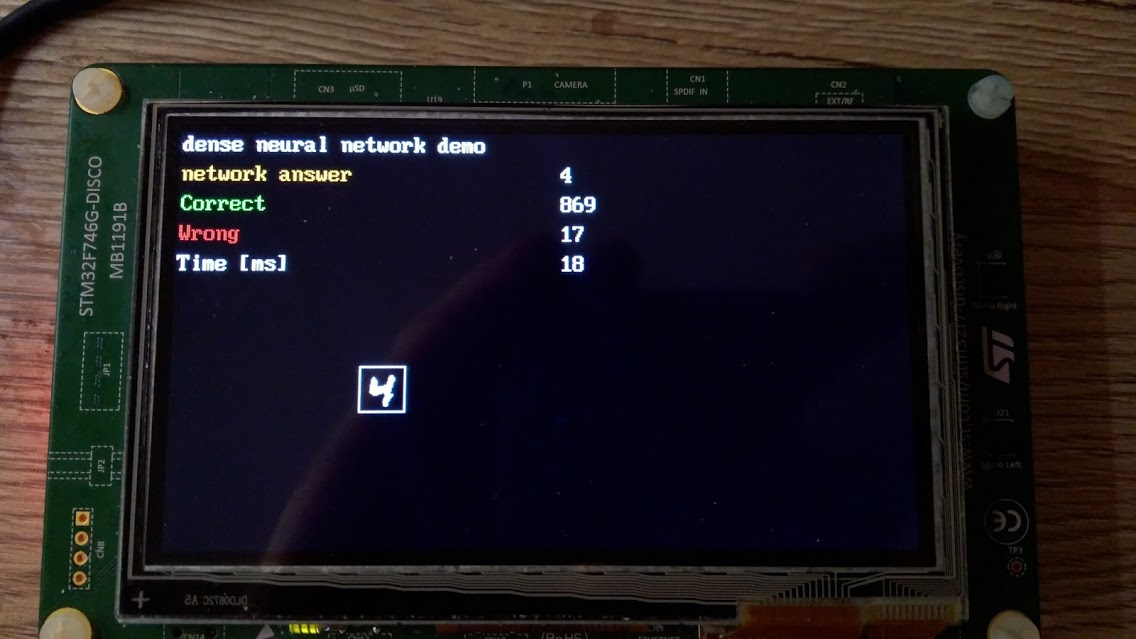
\includegraphics[scale=0.25]{../../pictures/stm32_screenshot.jpg}
\end{figure}

\end{frame}

\begin{frame}{\bf Usefull links}

{\tiny
  \begin{thebibliography}{9}
    \bibitem {}ImageNet Classification with Deep Convolutional Neural Networks \url{https://papers.nips.cc/paper/4824-imagenet-classification-with-deep-convolutional-neural-networks.pdf}
    \bibitem {}Alex Krizhevsky web, \url{https://www.cs.toronto.edu/~kriz/}
    \bibitem {}Deep Belief Nets in C++ and CUDA C: Volume III \url{https://www.amazon.com/Deep-Belief-Nets-CUDA-Convolutional/dp/1530895189}
    \bibitem {}Deep Learning (Adaptive Computation and Machine Learning \url{https://www.amazon.com/Deep-Learning-Adaptive-Computation-Machine/dp/0262035618}
    \bibitem {}Densely Connected Convolutional Networks \url{https://arxiv.org/pdf/1608.06993.pdf}

    \bibitem {}MNIST dataset \url{http://yann.lecun.com/exdb/mnist/}
    \bibitem {}Digital signal processing for STM32 microcontrollers using CMSIS \url{https://www.st.com/resource/en/application_note/dm00273990.pdf}

    \bibitem {}CMSIS-NN: Efficient Neural Network Kernels for Arm Cortex-M CPUs \url{https://arxiv.org/pdf/1801.06601.pdf}

  \end{thebibliography}
}

\end{frame}


\begin{frame}{\bf Q\&A}

\begin{figure}
  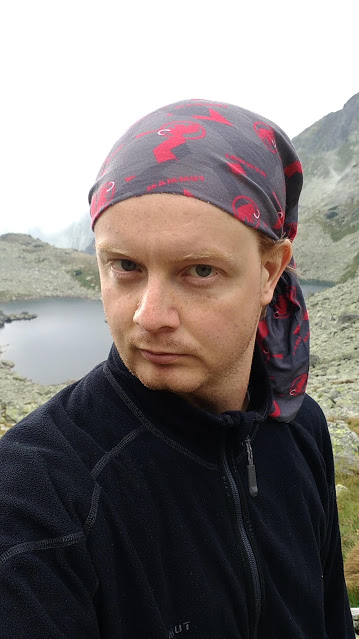
\includegraphics[scale=0.25]{../../pictures/me.jpg}
\end{figure}

\centering {
michal chovanec (michal.nand@gmail.com)
\url{www.youtube.com/channel/UCzVvP2ou8v3afNiVrPAHQGg}
}

\end{frame}


\end{document}




%% \bibitem {Deep Belief Nets in C++ and CUDA C: Volume III \url{https://www.amazon.com/Deep-Belief-Nets-CUDA-Convolutional/dp/1530895189}}
%% \bibitem {Deep Learning (Adaptive Computation and Machine Learning) \url{https://www.amazon.com/Deep-Learning-Adaptive-Computation-Machine/dp/0262035618}}
%% \bibitem {Densely Connected Convolutional Networks \url{https://arxiv.org/pdf/1608.06993.pdf}}
